\Solution{catMap}{soluCatMap}{23jan2018}{Cat map}
% siminos/spatiotemp/Solutions/soluCatMap.tex called by catMap.tex
% $Author: predrag $ $Date: 2021-08-10 11:56:19 -0400 (Tue, 10 Aug 2021) $

% Predrag                                               23jan2018

%%%%%%%%%%%%%%%%%%%%%%%%%%%%%%%%%%%%%%%%%%%%%%%%%%%%%%%%%%%%%%%%%%%
\solution{exer:catMapGreenInf}{Cat map Green's function, infinite lattice.}{

(a) It's just the roots of a quadratic equation, with
\(
s=\ExpaEig+\ExpaEig^{-1}
\,,
\)
and \(
\surd{D}=\ExpaEig-\ExpaEig^{-1}
\,.
\)


(b) The Green's function \refeq{GreenFun00b}
\beq
\gd_{tt'}=  \frac{1}{{\surd{D}}}\,\frac{1}{\ExpaEig^{|t'-t|}}
\ee{GreenFun00d}
for the discrete damped Poison
equation \refeq{eq:CatMapStep} was first computed explicitly by Percival and
Vivaldi\rf{PerViv}, using the methods introduced in Mestel and
Percival\rf{varcyc}. It should satisfy
\beq
(\D \gd)_{ij} = \sum_{k} \D_{ik} \gd_{kj} =\delta_{ij}
\,.
\ee{HLGFuncInf1}
Since we are considering infinite $1D$ lattice, we do not need to
specify the boundary conditions. $\D$ is a Toeplitz matrix
\beq
\D_{ik}=s \delta_{ik} - \delta_{i-1,k} - \delta_{i+1,k}
\ee{HLGFuncInf2}
Substituting \refeq{HLGFuncInf2} into \refeq{HLGFuncInf1}
\beq
\sum_{k} \D_{ik} \gd_{kj} = s \gd_{ij} -\gd_{i-1,j}-\gd_{i+1,j} =\delta_{ij}
\,,
\ee{HLGFuncInf3}
and substituting \refeq{GreenFun00b}
\beq
\gd_{ij}= \frac{1}{\surd{D}}\,
          \frac{1}{\ExpaEig^{|j-i|}}
=  \left\{ \begin{array}{ll}
\frac{1}{\surd{D}}\,\frac{1}{\ExpaEig^{i-j}}  & \mbox{ if } j < i  \\
\frac{1}{\surd{D}} & \mbox{ if } j = i  \\
\frac{1}{\surd{D}}\,\frac{1}{\ExpaEig^{j-i}}  & \mbox{ if } j > i
         \end{array}\right.
\,.
\ee{GreenFun00c}
into \refeq{HLGFuncInf3},
one verifies that \refeq{GreenFun00b} is indeed the Green's function
for the infinite lattice. By translational invariance, for $i=j$ consider
\beq
s \gd_{00} -\gd_{-1,0}-\gd_{10}
  = \frac{1}{\surd{D}}\,\left(
  {s} - \frac{2}{\ExpaEig}
     \right)
  = \frac{1}{\surd{D}}\,\left(\ExpaEig-\frac{1}{\ExpaEig}\right)
  = 1
\,.
\label{HLGFuncInf5}
\eeq
For $i>j$ consider
\beq
s \gd_{10} -\gd_{00}-\gd_{20}
  = \frac{1}{\surd{D}}\,\left(
  \frac{s}{\ExpaEig}
  - 1
  - \frac{1}{\ExpaEig^{2}}
     \right)
  = \frac{1}{\surd{D}}\,\frac{1}{\ExpaEig}
      \,\left( s - \ExpaEig-\frac{1}{\ExpaEig}\right)
  = 0
\,.
\label{HLGFuncInf4}
\eeq

(c) The orbit is recovered by:
\beq
\ssp_n=\sum_{n' \in \integers} \gd_{nn'} \Ssym{n'}
= \frac{1}{{\surd{D}}} \sum_{n' \in \integers} \ExpaEig^{- |n-n'|} \Ssym{n'}
\,.
\ee{HLGFuncInf6}
\hfill (Han Liang) %{2018-03-08}{
    } % end \solution{exer:catMapGreenInf}
%%%%%%%%%%%%%%%%%%%%%%%%%%%%%%%%%%%%%%%%%%%%%%%%%%%%%%%%%%%%%%%%%%%%%%%%

%%%%%%%%%%%%%%%%%%%%%%%%%%%%%%%%%%%%%%%%%%%%%%%%%%%%%%%%%%%%%%%%%%%
\solution{exer:catMapGreenPBC}{Cat map Green's function for a \po.}{
%    \PC{2017-08-28} {
%``Average coordinate'' depends on b.c.'s. Average coordinate
%\refeq{catMapAverCoord} is computed for
%the the very unphysical Dirichlet boundary condition $\ssp_z=0$ for $z\in \R$
%which breaks translation invariance.
%If one takes the much gentler, translationally invariant doubly periodic b.c.,
%the ``average coordinate'' $\bar{x}_z$ is the \twot\ periodic point, a
%more natural choice.
%    }
Express the periodic orbit Green's function in terms of the infinite
lattice by using a periodic source $\Ssym{n'}=\Ssym{n'}+\cl{p}$,
\bea
\sum_{n'=-\infty}^{\infty}\gd_{nn'}\Ssym{n'}
 &=& \sum_{r=-\infty}^{\infty} \sum_{n'=r\cl{p}}^{r\cl{p}+\cl{p}-1}\gd_{nn'}\,\Ssym{n'}
= \sum_{r=-\infty}^{\infty} \sum_{n'=0}^{\cl{p}-1}\gd_{n,n'+r\cl{p}}\,\Ssym{n'+r\cl{p}}
\continue
 &=& \sum_{r=-\infty}^{\infty} \sum_{n'=0}^{\cl{p}-1}\gd_{n-n',r\cl{p}}\,\Ssym{n'}
\label{HLGFuncPO1}
\eea
Comparing with the expression for the Green's function of a periodic orbit:
\beq
\sum_{n'=0}^{\cl{p}-1}\gd_{nn'}^\cl{p} \Ssym{n'}
\label{HLGFuncPO2}
\eeq
we see that
\beq
\gd_{nn'}^\cl{p}=\sum_{r=-\infty}^{\infty} \gd_{n-n',r\cl{p}}
\ee{HLGFuncPO3}
Substituting \refeq{GreenFun00b} into \refeq{HLGFuncPO3} we have:
%\beq
%	\gd_{n,n'}^P
%	&=& \frac{1}{\surd{D}}\sum_{r=-\infty}^{\infty} \frac{1}{\ExpaEig^{|n-n'-rP|}}
%\ee{HLGFuncPO4}
% HL could not print this. PC should have used \bea ... \label{HLGFuncPO4}\eea
\bea
   \gd_{nn'}^\cl{p}
   &=& \frac{1}{\surd{D}}\sum_{r=-\infty}^{\infty} \frac{1}{\ExpaEig^{|n-n'-r\cl{p}|}}
   \continue
   &=& \frac{1}{\surd{D}} \left( \frac{1}{\ExpaEig^{|n-n'|}}
   +\sum_{r=1}^{\infty} \frac{1}{\ExpaEig^{r\cl{p}-(n-n')}}
   + \sum_{r=-1}^{-\infty} \frac{1}{\ExpaEig^{(n-n')-r\cl{p}}}
   \right)
   \continue
   &=& \frac{1}{\surd{D}} \left(  \frac{1}{\ExpaEig^{|n-n'|}}
   +\frac{1}{\ExpaEig^{-|n-n'|}}\frac{1}{\ExpaEig^\cl{p}-1}
   +\frac{1}{\ExpaEig^{|n-n'|}}\frac{1}{\ExpaEig^\cl{p}-1}
   \right)
   \continue
   &=& \frac{1}{\surd{D}}\,
       \frac{1}{1-\ExpaEig^{-\cl{p}}}
       (\ExpaEig^{-|n-n'|} + \ExpaEig^{-\cl{p}+|n-n'|})
   \label{HLGFuncPO4}
\eea
This verifies \refeq{GreenFun2}.

Bird and Vivaldi\rf{BirViv} show that for an $n$-cycle $\ssp_{n'}$ are
rational functions of $\ExpaEig$, given by the quotient of two reflexive
polynomials
(for example, $P_t(\ExpaEig)= \ExpaEig^n P_t(1/\ExpaEig)$),
\bea
\ssp_{t} &=&  \ExpaEig \,{P_t(\ExpaEig)}/{Q(\ExpaEig)}
        \continue
P_t(\ExpaEig) &=&  \sum_{\tau=1}^{n-1}
                   \ExpaEig^{n-\tau}(\ExpaEig\,\Ssym{t+\tau-1} + \Ssym{t-\tau})
        \continue
Q(\ExpaEig) &=&  (\ExpaEig^2 - 1)\,(\ExpaEig^n - 1)
\label{BirViv(3.5)a}
\eea
Bird and Vivaldi\rf{BirViv} then discuss pruning, give formulas for the
numbers of {\orbit}s for integer $s$, \etc.

\hfill (Han Liang) %{2018-03-08}
    } % end \solution{exer:catMapGreenPBC}
%%%%%%%%%%%%%%%%%%%%%%%%%%%%%%%%%%%%%%%%%%%%%%%%%%%%%%%%%%%%%%%%%%%%%%%%

%%%%%%%%%%%%%%%%%%%%%%%%%%%%%%%%%%%%%%%%%%%%%%%%%%%%%%%%%%%%%%%%%%%
\solution{exer:catMapGreend=2wrong}{$d=2$ cat map guess Green's function, infinite lattice.}{
% \HLpost{2018-03-12}{ The Green's function \refeq{GreenFund=2wrong} is not correct.
The Green's function $\gd$ for the Toeplitz matrix (tensor) in 2 dimensions
\bea
\D_{lt,l't'} &=& \left[-\Box + 2\left({s}/{2} - 2\right)\right]_{lt,l't'}
\continue
&=& \left(\frac{s}{2}\delta_{ll'}-\delta_{l-1,l'}-\delta_{l+1,l'}\right)\delta_{tt'}
\ceq
   +\delta_{ll'}\left(\frac{s}{2}\,\delta_{tt'}-\delta_{t-1,t'}-\delta_{t+1,t'}\right)
\,.
\label{HLGreenFund=2B}
\eea
should satisfy \refeq{HLGreenFund=2C},
or, substituting \refeq{HLGreenFund=2B} into \refeq{HLGreenFund=2C},
\bea
\PCedit{2\,}
\delta_{ll'}\delta_{tt'}
   &=& \frac{s}{2}\gd_{ll',tt'}-\gd_{l-1,l',tt'}-\gd_{l+1,l',tt'}
\ceq
     + \frac{s}{2}\gd_{ll',tt'}-\gd_{ll',t-1,t'}-\gd_{ll',t+1,t'}
\,.
\label{HLGreenFund=2D}
\eea
Let's check this.
By translational invariance, need to look only at different values of
$l-l'$ and $t-t'=0$. For $l=l'$ and $t=t'$ it suffices that we consider
the $l=l'=t=t'=0$ case. Using \refeq{catEigsEx2D} we have
\bea
&&\frac{s}{2} \gd_{00,00} -\gd_{-1,0,00}-\gd_{10,00}
\ceq
+ \frac{s}{2} \gd_{00,00} -\gd_{00,-1,0}-\gd_{00,10}
\ceq
  = \frac{2}{\surd{D}}\,\left(
    \frac{s}{2} - \frac{2}{\ExpaEig}
     \right)
  = \frac{2}{\surd{D}}\,\left(\ExpaEig-\frac{1}{\ExpaEig}\right)
  = 2
\,,
\label{HLGFuncInf5a}
\eea
verifies \refeq{HLGreenFund=2B}.

For $l>l'$ and $t=t'$ it suffices
to consider $l=1,l'=0$, $t=t'=0$  case.
\bea
&&\frac{s}{2} \gd_{10,00} -\gd_{00,00}-\gd_{20,00}
    \ceq
 + \frac{s}{2} \gd_{10,00} -\gd_{10,-1,0}-\gd_{10,10}
\ceq
  = \frac{1}{2\surd{D}}\,\left(
  \frac{s/2}{\ExpaEig}
  - 1
  - \frac{1}{\ExpaEig^{2}}
     \right)
  + \frac{1}{2\surd{D}}\,\left(
  \frac{s/2}{\ExpaEig}
   - \frac{2}{\ExpaEig^{2}}
     \right)
\ceq
  = \frac{1}{2\ExpaEig\surd{D}}\,\left(
        \frac{s}{2} - \frac{2}{\ExpaEig^{}}
     \right)
  = \frac{1}{2\ExpaEig\surd{D}}
      \,\left(\ExpaEig-\frac{1}{\ExpaEig}\right)
  = \frac{1}{2\ExpaEig}
\,.
\label{HLGFuncInf4b}
\eea
%\PCedit{2017-03-15 Han is right,
So, the guess \refeq{GreenFund=2wrong} already does not work.

Substitute \refeq{GreenFund=2wrong} into \refeq{HLGreenFund=2D} we get:
\bea
\sum_{z''}\D_{zz''}\gd_{z''z'}
=  \left\{ \begin{array}{ll}
\frac{1}{\surd{D}}\,\frac{1}{\ExpaEig^{|\ell'-\ell|+|t'-t|}} (s-2\ExpaEig-2\ExpaEig^{-1})
           & \mbox{ if } l\neq l'\,and\,t\neq t'   \\
\frac{1}{\surd{D}} (s-4\ExpaEig^{-1})
           & \mbox{ if } l=l'\, and\, t=t'
         \end{array}\right.
\,.
\label{HLGreenFund=2E}
\eea

To satisfy \refeq{HLGreenFund=2C}, $s$, $\surd{D}$ and $\ExpaEig$ must satisfy:
\bea
\left\{ \begin{array}{ll}
s=2\ExpaEig+2\ExpaEig^{-1} \\
\surd{D} = 2\ExpaEig-2\ExpaEig^{-1}
         \end{array}\right.
\,.
\label{HLGreenFund=2F}
\eea
So we will have:
\bea
\left\{ \begin{array}{ll}
\ExpaEig = \frac{1}{4}(s+\sqrt{s^2-16})\\
\ExpaEig^{-1} = \frac{1}{4}(s-\sqrt{s^2-16})
         \end{array}\right.
\,.
\label{HLGreenFund=2G}
\eea
Now the problem is, if $l \neq l'$ but $t = t'$, \refeq{HLGreenFund=2E} become:
\beq
\sum_{z''}\D_{zz''}\gd_{z''z'}
  = \frac{1}{\surd{D}}\,\frac{1}{\ExpaEig^{|\ell'-\ell|+|t'-t|}} (s-\ExpaEig-3\ExpaEig^{-1})
\ee{HLGreenFund=2H}
and this is not satisfied by \refeq{HLGreenFund=2G}. So
\refeq{GreenFund=2wrong} does not work for the 2-dimensional case. I
haven't figured out the correct Green's function for the 2 dimensions.

\hfill (Han Liang) %{2018-03-12}
    } % end \solution{exer:catMapGreend=2wrong}
%%%%%%%%%%%%%%%%%%%%%%%%%%%%%%%%%%%%%%%%%%%%%%%%%%%%%%%%%%%%%%%%%%%%%%%%

%%%%%%%%%%%%%%%%%%%%%%%%%%%%%%%%%%%%%%%%%%%%%%%%%%%%%%%%%%%%%%%%%%%
\solution{exer:catMapGreend=2wrong}{$d=2$ cat map guess Green's function, infinite lattice.}{
%\HLpost{2018-03-15}{
The guess Green's function \refeq{GreenFund=2wrong} doesn't work.
For $l=2$, $l'=0$ and $t=t'=0$, the correct form of \refeq{HLGFuncInf4b} is:
\bea
&&\frac{s}{2} \gd_{10,00} -\gd_{00,00}-\gd_{20,00}
\ceq
+ \frac{s}{2} \gd_{10,00} -\gd_{10,10}-\gd_{10,-10}
\\
  &=& \frac{1}{2\surd{D}}\,\left(
  \frac{s}{2\ExpaEig}
  - 1
  - \frac{1}{\ExpaEig^{2}}
     \right)+
     \frac{1}{2\surd{D}}\,\left(
  \frac{s}{2\ExpaEig}
  - \frac{1}{\ExpaEig^{2}}
  - \frac{1}{\ExpaEig^{2}}
     \right)
   \\
  &=& \frac{1}{2\surd{D}}\,\frac{1}{\ExpaEig}
      \,\left( \frac{s}{2} - \ExpaEig-\frac{1}{\ExpaEig}\right)
      +\frac{1}{2\surd{D}}\,\frac{1}{\ExpaEig}\,\left(
  \frac{s}{2}
  - \frac{1}{\ExpaEig}
  - \frac{1}{\ExpaEig}
     \right)\\
  &=& 0 + \frac{1}{2\ExpaEig}
\,.
\label{HLGFuncInf4I}
\eea
%\PCedit{2017-03-15
As in \refeq{HLGFuncInf4b}, this does not work .

\hfill (Han Liang) %{2018-03-12}
    } % end \solution{exer:catMapGreend=2wrong}
%%%%%%%%%%%%%%%%%%%%%%%%%%%%%%%%%%%%%%%%%%%%%%%%%%%%%%%%%%%%%%%%%%%%%%%%


%%%%%%%%%%%%%%%%%%%%%%%%%%%%%%%%%%%%%%%%%%%%%%%%%%%%%%%%%%%%%%%%%%%
\solution{exer:AKScatMapPOs}{\Po s of Arnol'd cat map.}{
No solution available.
} % end \solution{e-trajectNotIntersect}
%%%%%%%%%%%%%%%%%%%%%%%%%%%%%%%%%%%%%%%%%%%%%%%%%%%%%%%%%%%%%%%%%%%

%%%%%%%%%%%%%%%%%%%%%%%%%%%%%%%%%%%%%%%%%%%%%%%%%%%%%%%%%%%%%%%%%%%
\solution{exer:n=2GenPart}{The second iterate generating partition.}{
%	\HLpost{2019-08-10}{
\refFig{fig:PVAdlerWeiss2Steps} is the generating partition with $s=3$
evolved after 2 steps. In the Markov diagram
\reffig{fig:PVAdlerWeiss2Steps}\,(d) there are 7 self cycles, two of which
are the over-counted fixed points at the origin. So there are actually 5
periodic points with period 2, including 1 fixed point and 2 length-2
{\orbit}s, as given by \refeq{noPrimeCycs=3}.

%%%%%%%%%%%%%%%%%%%%%%%%%%%%%%%%%%%%%%%%%%%%%%%%%%%%%%%%%%%%
	\begin{figure}\begin{center}
            \begin{minipage}[c]{0.36\textwidth}\begin{center}
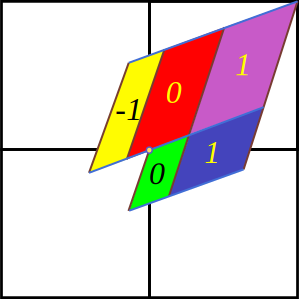
\includegraphics[width=1.0\textwidth]{PVAdlerWeissB-c}\\(a) %{PVAdlerWeiss2Steps-a}\\(a)
\\
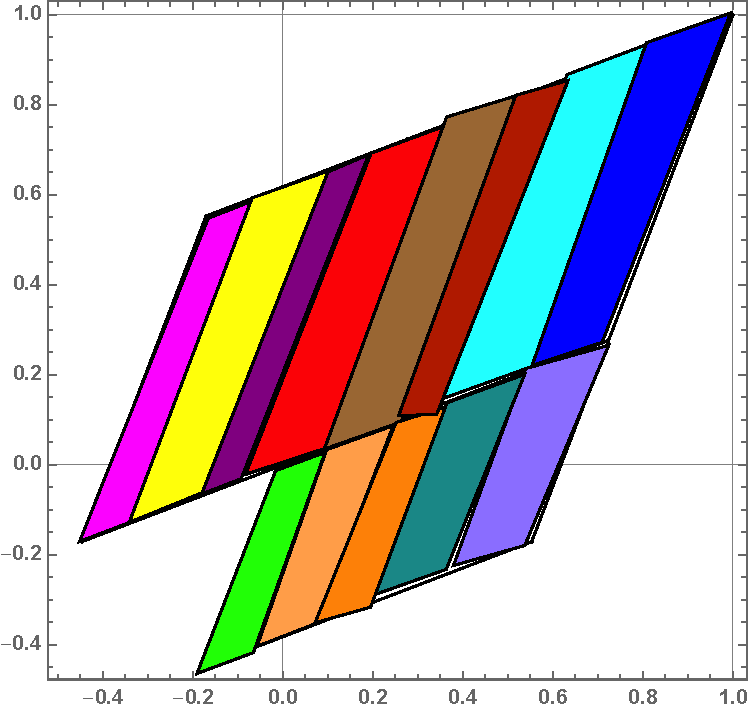
\includegraphics[width=1.0\textwidth]{PVAdlerWeiss2Steps-c}\\(c)
            \end{center}\end{minipage}
            \begin{minipage}[c]{0.3\textwidth}\begin{center}
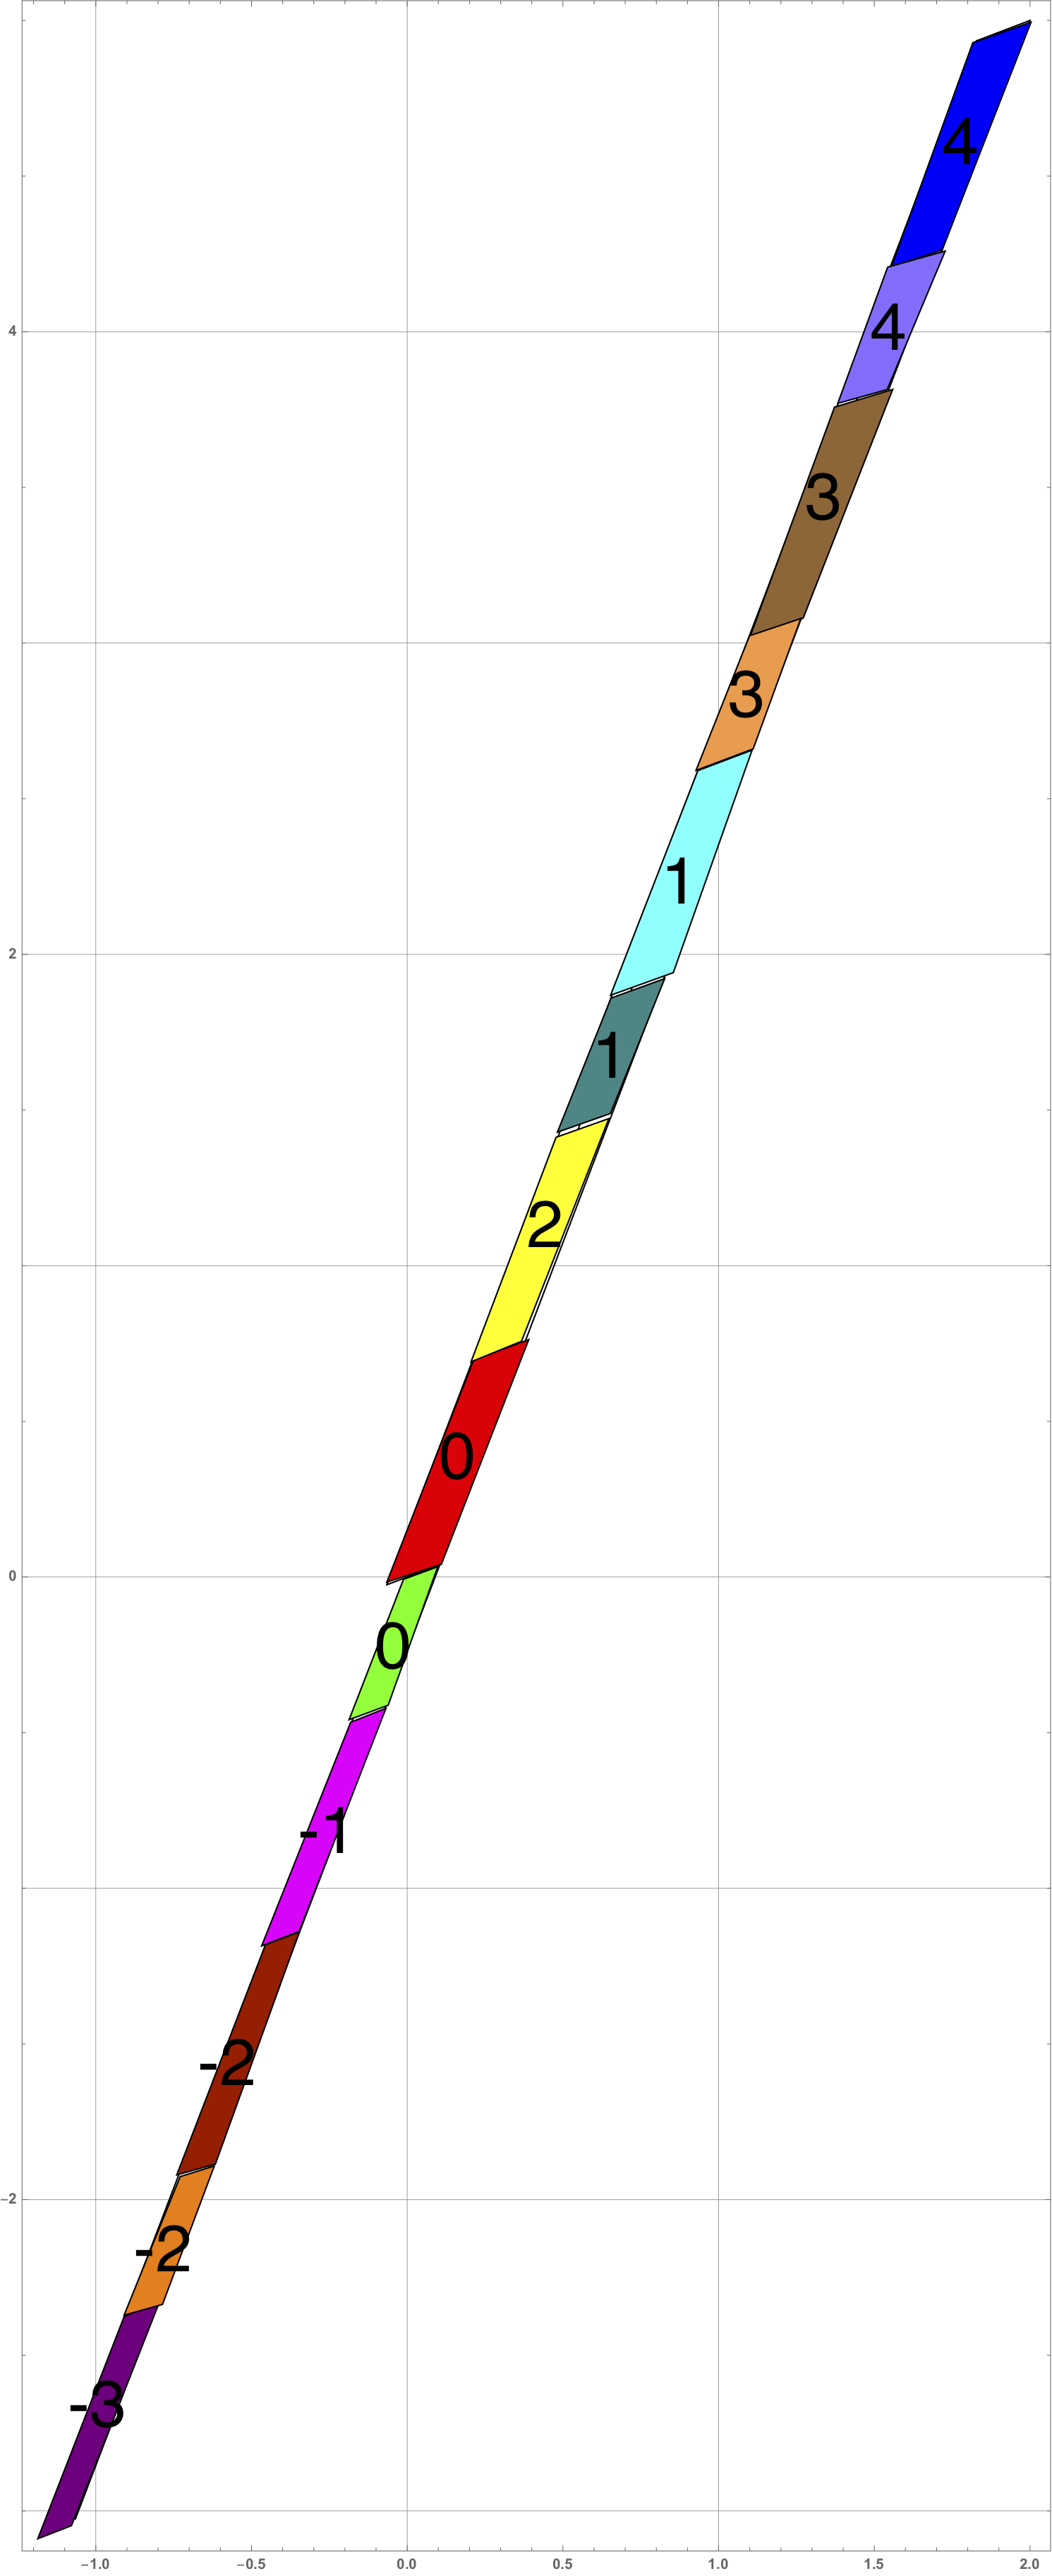
\includegraphics[width=1.0\textwidth]{PVAdlerWeiss2Steps-b}\\(b)
            \end{center}\end{minipage}
            ~~~
            \begin{minipage}[c]{0.25\textwidth}\begin{center}
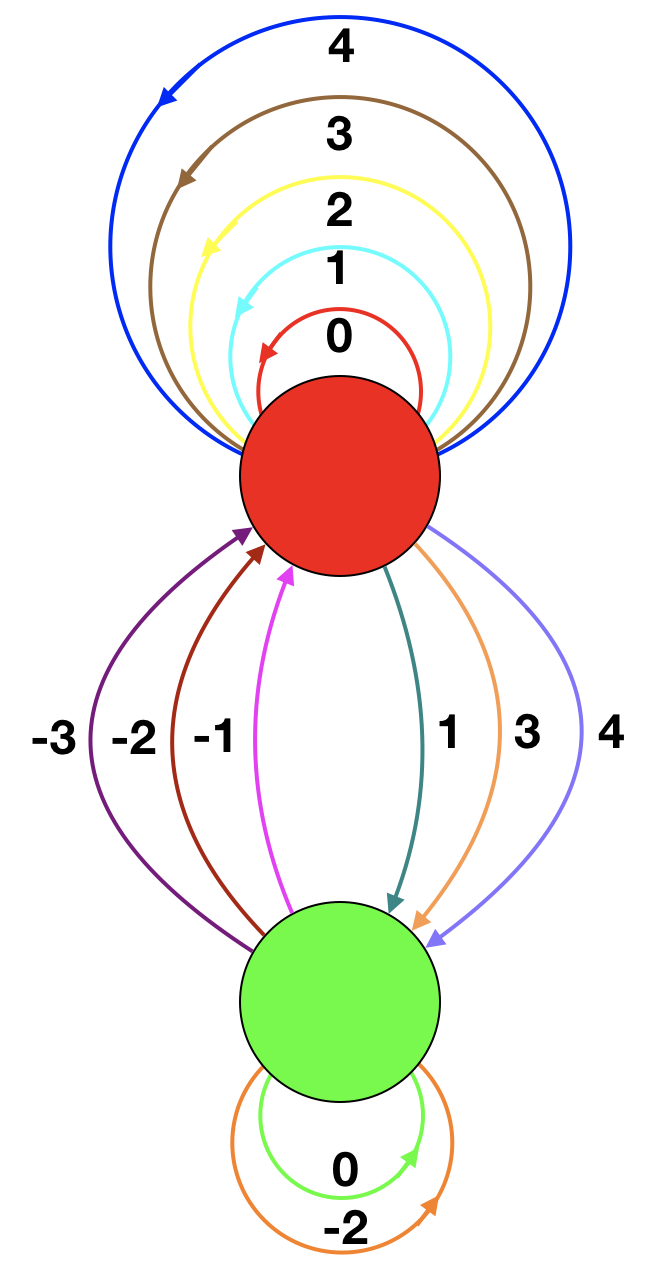
\includegraphics[width=1.0\textwidth]{PVAWMarkov2Steps}\\(d)
            \end{center}\end{minipage}
\end{center}
  \caption{\label{fig:PVAdlerWeiss2Steps}
(a)
An \AW\ one step forward in time partition of the unit torus for the
$s=3$ \PV\ cat map \reffig{fig:PVAdlerWeissB}\,(c).
(b)
Mapped two steps forward in time, the rectangles are stretched along the
unstable direction and shrunk along the stable direction. Sub-rectangles
$\pS_j$ that have to be translated back into the partition are indicated by
color and labeled by their lattice translation
$\Ssym{j}$.
(c)
The sub-rectangles $\pS_j$ translated back into the unit square yield a
two steps forward in time
generating partition (a subpartition of rectangles in (a)), with
(d)
the finite grammar given by the {\markGraph} for this partition. The nodes
refer to the rectangles $A$ and $B$, and the 13 links correspond to the 13
sub-rectangles induced by two step forward-in-time dynamics.
}
\end{figure}
%%%%%%%%%%%%%%%%%%%%%%%%%%%%%%%%%%%%%%%%%%%%%%%%%%%%%%%%%%%%

%%%%%%%%%%%%%%%%%%%%%%%%%%%%%%%%%%%%%%%%%%%%%%%%%%%%%%%%%%%%%
\begin{figure}
  \centering
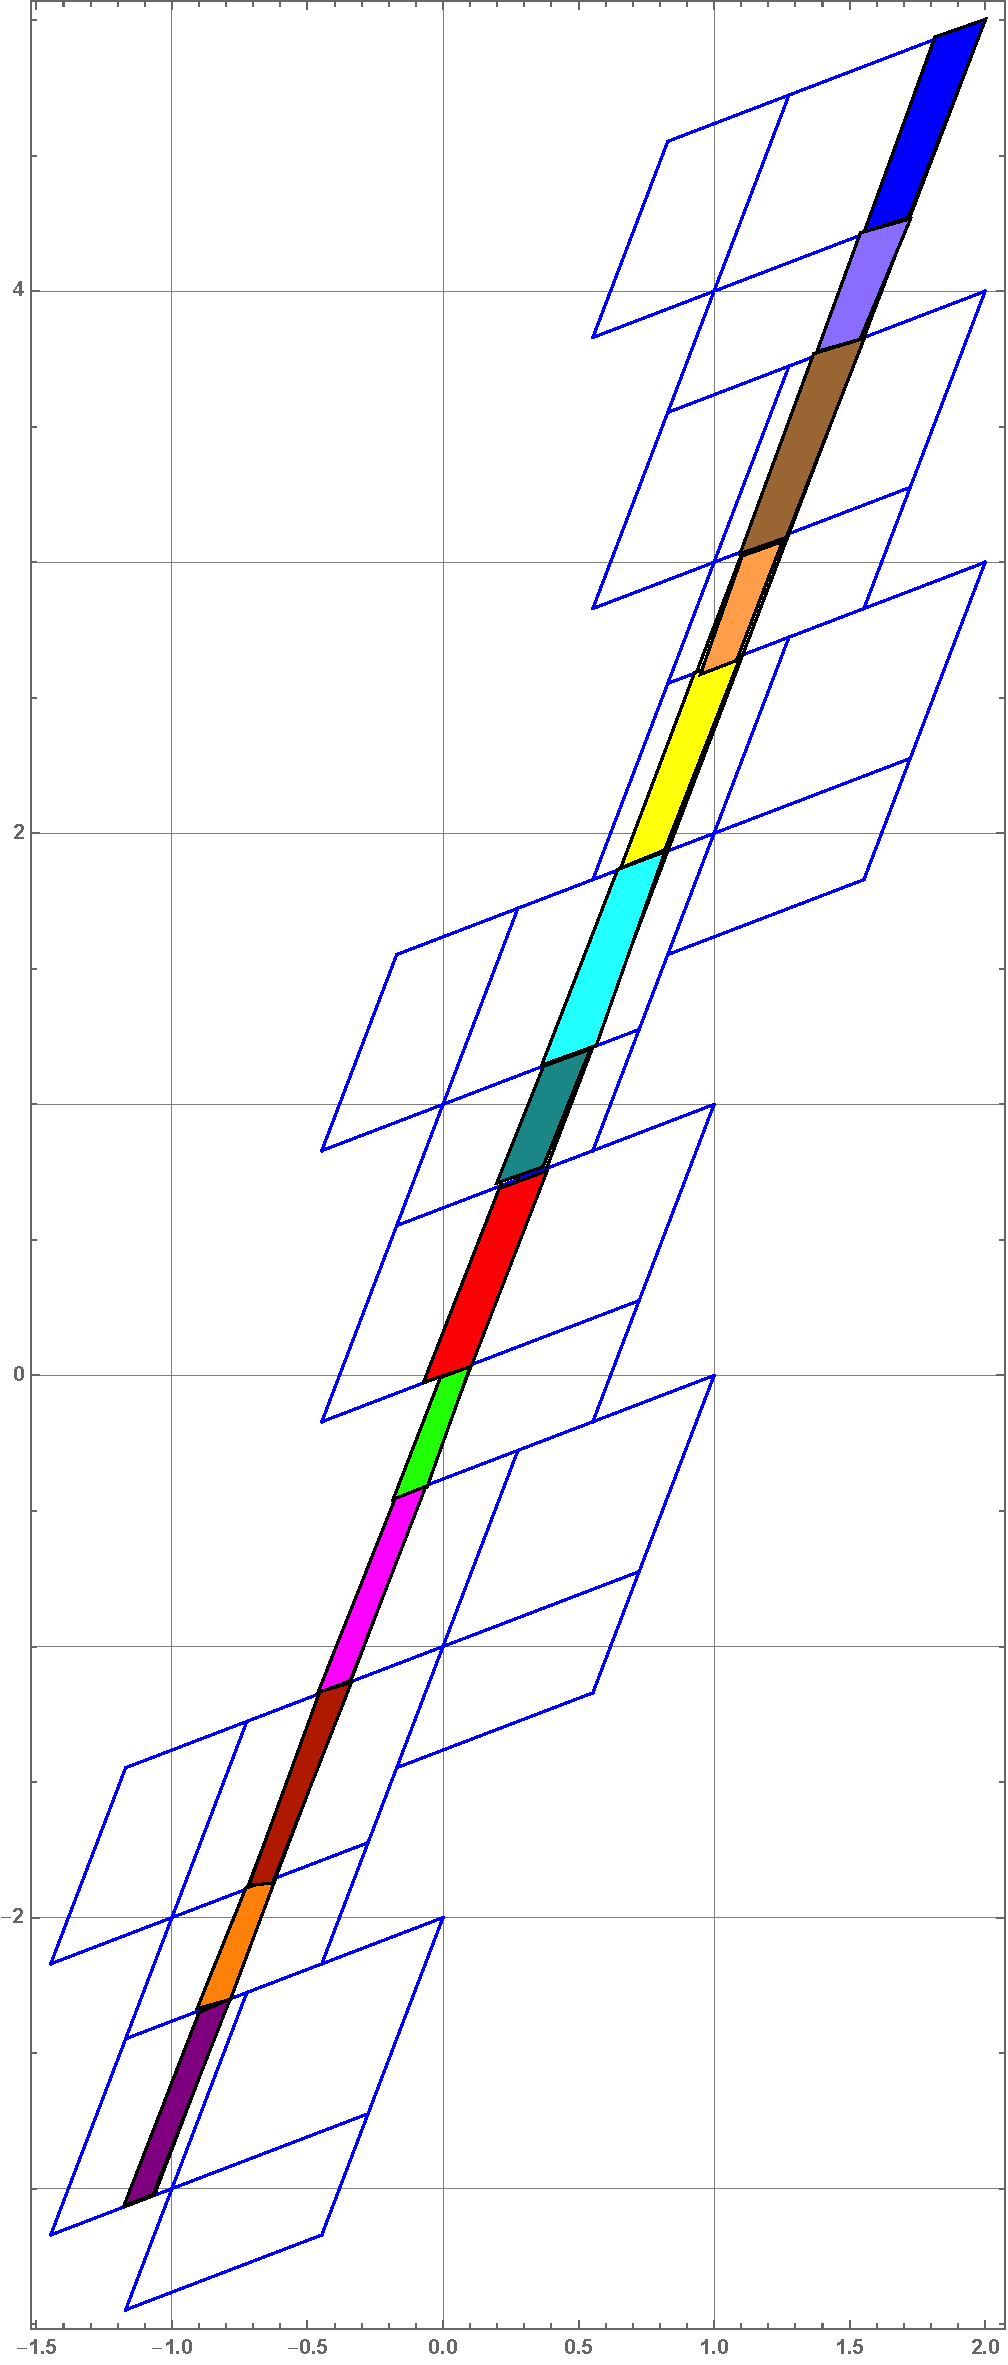
\includegraphics[width=0.40\textwidth]{PVAdlerWeiss2Steps-d}
  \caption{\label{fig:PVAdlerWeiss2StepsD}
This figure is used to track where each sub-rectangles in
\reffig{fig:PVAdlerWeiss2Steps} goes. Note that two step forward-in-time
requires both vertical and horizontal shifts, unlike the one step
forward-in-time \PV\ cat map \refeq{eq:StateSpCatMap}.
}
\end{figure}
%%%%%%%%%%%%%%%%%%%%%%%%%%%%%%%%%%%%%%%%%%%%%%%%%%%%%%%%%%%%%%%

\refFig{fig:PVAdlerWeiss2Steps} is a very nice illustration
of a generating partition subrectangles being further subdivided.
} % end \solution{exer:n=2GenPart}
%%%%%%%%%%%%%%%%%%%%%%%%%%%%%%%%%%%%%%%%%%%%%%%%%%%%%%%%%%%%%%%%%%%
